\section{Results}\label{sec:results}

SMA-based partitioning of performance observations provides a procedural method for grouping time-correlated performance events observed during this experiment.
In the following sections, we identify regions at different timescales and apply several statistical methods over these regions to identify the breadth of performance anomalies that occur on large-scale production file systems.

\subsection{Long-term performance evolution} \label{sec:results/longterm}

\begin{figure}[t]
    \centering
    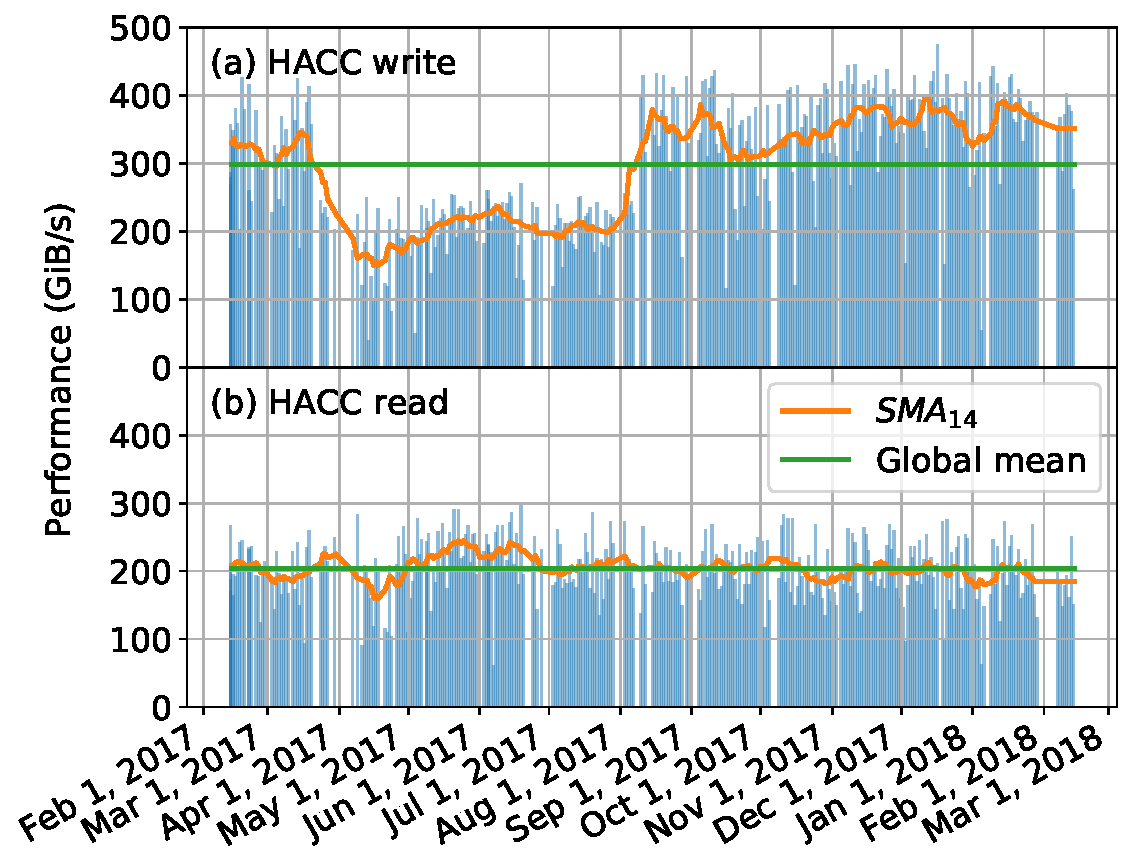
\includegraphics[width=1.0\columnwidth]{longterm-cscratch-hacc}
    \vspace{-.35in}
    \caption{Performance evolution of HACC file-per-process workload on Cori.  Red line is the overall mean (298 GiB/sec write, 204 GiB/sec read) and blue bars are raw performance measurements.}
    \label{fig:timeseries-baseline}
    % source: sc18_segments.ipynb
\end{figure}

The horizontal bands in Figures \ref{fig:summary-heatmap} and \ref{fig:regions-heatmap}b identify long periods of reduced performance for the file-per-process write workloads as dark horizontal bands between April and August.
Because this region occurred over a period of months, we choose a ${w_{short}} = 14$ days to minimize the effects of high-frequency transients and ${w_{long}} \rightarrow \infty$ to identify divergence regions that are abnormal relative to the global mean performance.  The resulting SMAs for the HACC write workload on Cori are shown in Figure \ref{fig:timeseries-baseline}a.

The crossovers between $\textup{SMA}_{14}$ and $\textup{SMA}_{\infty}$ visibly distinguish the extent of the long-term performance depression that occurred between April and August for the HACC write workload.
The divergence region defining this performance depression lasted for 139 days, and no other divergence regions were identified for this workload.
In stark contrast, the performance of HACC read workload (Figure \ref{fig:timeseries-baseline}b) was unaffected during this time; the longest divergence region identified was 59 days long and exhibited abnormally \emph{high} performance.
Incidentally, this abnormally high performance occurred between May 7 and July 4--a time when the HACC write performance was also experiencing high performance \emph{relative to its long-term performance depression.}

These data demonstrate that the nominal peak performance of specific applications' I/O can vary over the service life of a storage system and its dependent components.
Furthermore, the difference between the read and write motifs in Figure \ref{fig:timeseries-baseline} indicates that not all workloads are affected by long-term variation equally. 
In this case of HACC on Cori, write performance was adversely for a period of months while read performance of the same I/O pattern was completely unaffected.

In combination with expert knowledge, the root cause for the long-term performance depression in the HACC write workload was retrospectively identified using the boundaries of the 139-day divergence region.
The intersection between $\textup{SMA}_{14}$ and $\textup{SMA}_\infty$ in Figure \ref{fig:timeseries-baseline} occurs at March 24 and August 10, and comparing these dates to the service history of Cori revealed that operating system upgrades occurred on exactly those dates--March 24 and August 10.
The Lustre client versions were updated on those two dates, and the appearance and subsequent disappearance of the anomalous behavior was attributed to a bug in the client software.
% March 24 was the upgrade of CLE6UP01 to UP03, and August 10 was CLE6UP03 to UP04.  The performance loss in t > Aug 10 is caused by Lustre bug LU-9574
\TODO{Has this bug affected IOR/fpp R/W the same way? That could confirm (to some extent) that all apps with similar I/O patterns might have suffered from this bug. Has this bug affected shared file patterns similarly? -- Suren

Glenn: Yes, Figure \ref{fig:regions-heatmap}b shows that ior/fpp/write was also affected, but none of the other benchmarks were.}
Finally, our choice of averaging $\textup{SMA}_{short}$ over ${-0.5w_{short} <= t < +0.5w_{short}}$ makes it insensitive to choice of $w_{short}$.
For this dataset, changing $\textup{SMA}_{short}$ from $\textup{w}_{14}$ to both $\textup{w}_{7}$ and $\textup{w}_{28}$ resulted in no change to the dates bounding the 139-day divergence region.
The principal effect of changing $\textup{w}_{short}$ is the number of short regions that arise from the higher-frequency oscillations of $\textup{SMA}_{short}$ around $\textup{SMA}_{long}$.





\subsection{Transitions between divergence regions} \label{sec:results/transitions}

\begin{figure}
    \centering
    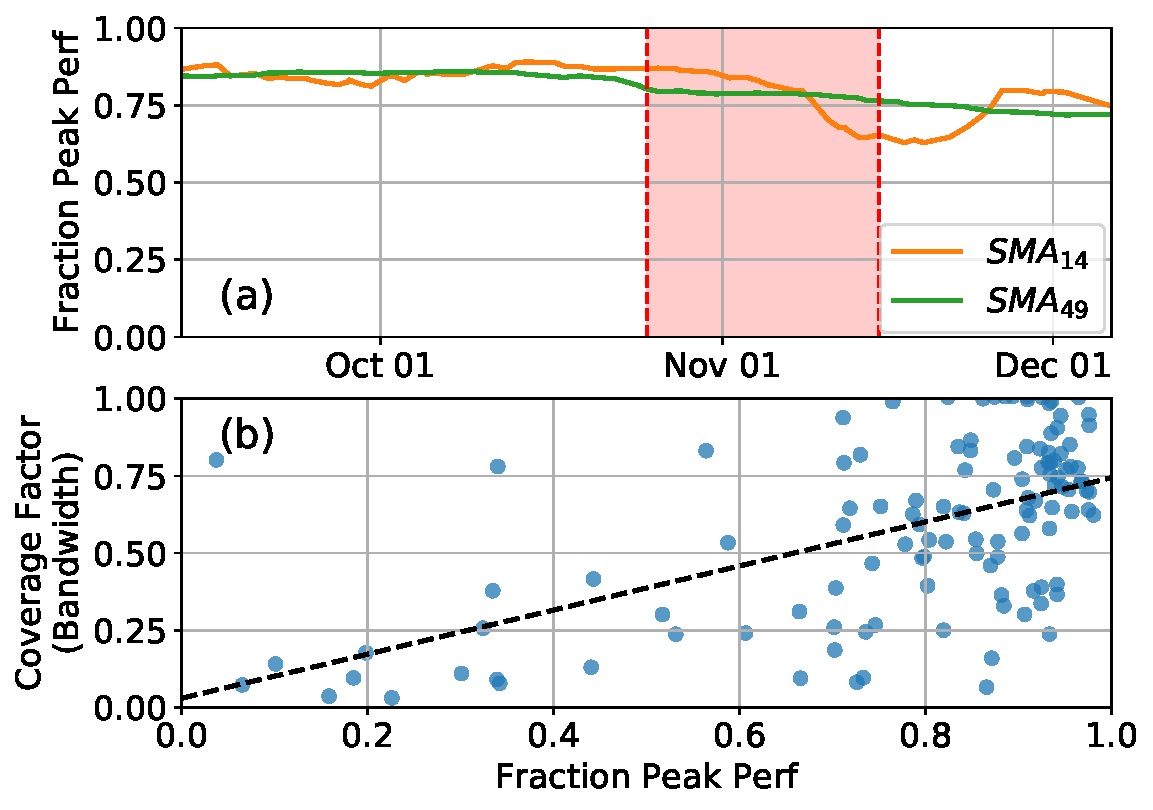
\includegraphics[width=1.0\columnwidth]{mira-correlation-region}
    \vspace{-.35in}
    \caption{Correlation between performance and $CF_{bw}$ in a transition between divergence regions on Mira. (a) shows a region automatically detected using the centroid method, and (b) shows the correlation between performance and $CF_{bw}$ in that region.  Correlation coefficient is $0.565$ and p-value is ${1.48 \times 10^{-11}}$; dashed line in (b) is a linear fit with slope $0.714$ drawn for visual aid.}
    \label{fig:mira-correlation-region}
    % source: sc18_centroids-for-paper.ipynb
\end{figure}

%Long-term behavior has very low frequency by definition, so analyzing the causes of a few long-term performance depressions by hand (as was done in Section \ref{sec:results/longterm}) is not unreasonable.
%With smaller values of $w_{long}$, though, this method identifies an increasing number of divergence regions, and characterizing the factors that contribute to these long-term performance depressions using automated statistical techniques becomes imperative.

Performance can be effectively correlated with other metrics collected during I/O-intensive jobs if sufficient variation in performance is observed in the neighboring jobs to establish compelling correlation coefficients.
To capture regions that exhibit a broad range of performance measurements, we convert pairs of divergence regions into \emph{trend regions} as defined in Section \ref{sec:features}.

%We then discard divergence regions whose $\textup{SMA}_{short}$ exhibit minimal change between their first and last value in the region.  For each divergence region bounded by times $t_0$ and $t_f$, we then discard those regions where
%
%\begin{equation}
%abs \left (
%\frac
%	{ \textup{SMA}_{short}(t_0) - \textup{SMA}_{short}(t_f) }
%	{\textup{SMA}_{short}(t_f)}
%\right ) < C
%\end{equation}
%
%and $C$ is a cutoff threshold typically between 0.15 and 0.40 whose optimal value is a function of $w_{short}$, $w_{long}$, and how variable the storage system performance tends to be over long periods of time.
%Given a well-chosen $C$, the result set of divergence regions satisfy both the (\ref{sec:results/transitions/criterion1}) sampling criterion and (\ref{sec:results/transitions/criterion2}) diversity criterion.

To demonstrate the utility of this approach, we apply it to the entirety of performance observations across all benchmarks run on Mira.
It identifies eleven divergence regions across the entire year, and for each of these trend regions, we then calculate the Pearson correlation coefficient between the fraction peak performance observations and the other telemetric data associated with each job as described in Section \ref{sec:methods/tokio}.

Discarding all correlations except those with extremely high confidence ($\textup{p-value} > {1.0 \times 10^{-5}}$), only five of the eleven regions exhibited moderate correlation ($R > 0.35$) between performance and any other metric.
Furthermore, the bandwidth coverage factor was the sole metric that showed compelling correlation with performance in these five regions, with correlation coefficients ranging from +0.399 to +0.590.

An example of one of these regions and the correlation between performance and bandwidth coverage factor observed within is shown in Figure \ref{fig:mira-correlation-region}.
During this region, $\textup{SMA}_{short}$ fell from a 0.868 fraction of peak performance to 0.654 over 21 days, representing a significant loss of performance.
While this correlative analysis cannot attest to the cause of this event, this analysis confidently identified a long-term performance transition between October 25 and November 15 that was strongly correlated ($R = 0.565$) with bandwidth contention.
The fact that this correlation with performance degradation was observed across all I/O motifs (similar to Figure \ref{fig:regions-heatmap}a) distinguishes it from the case discussed in section \ref{sec:results/longterm} and further indicates a system-wide loss of performance.
The relative rarity of an event of this magnitude on Mira further suggests that the contentious activity coincident with this performance depression on Mira was likely not caused by routine job traffic and may have been related to year-end activity on the system.







\subsection{Transient performance loss} \label{sec:results/shortterm}

\begin{figure}
    \centering
    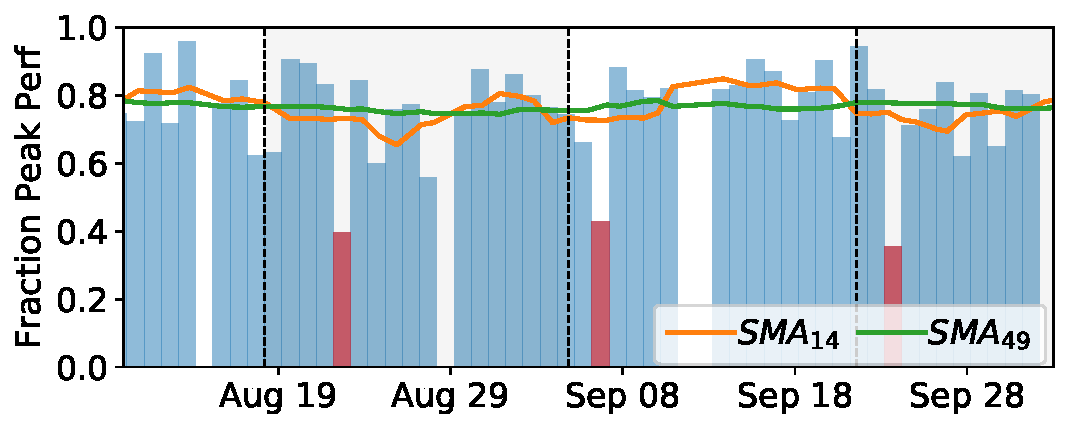
\includegraphics[width=1.0\columnwidth]{shortterm-mirafs1-dbscan}
    \vspace{-.35in}
    \caption{SMA partitioning and using minima in each region to identify transient.  The region from August 30 to September 5 contained fewer than seven measurements, so it was not considered.}
    \label{fig:shortterm-mirafs1-dbscan}
    % source: sc18_umamify.ipynb
\end{figure}

\begin{figure}
    \centering
    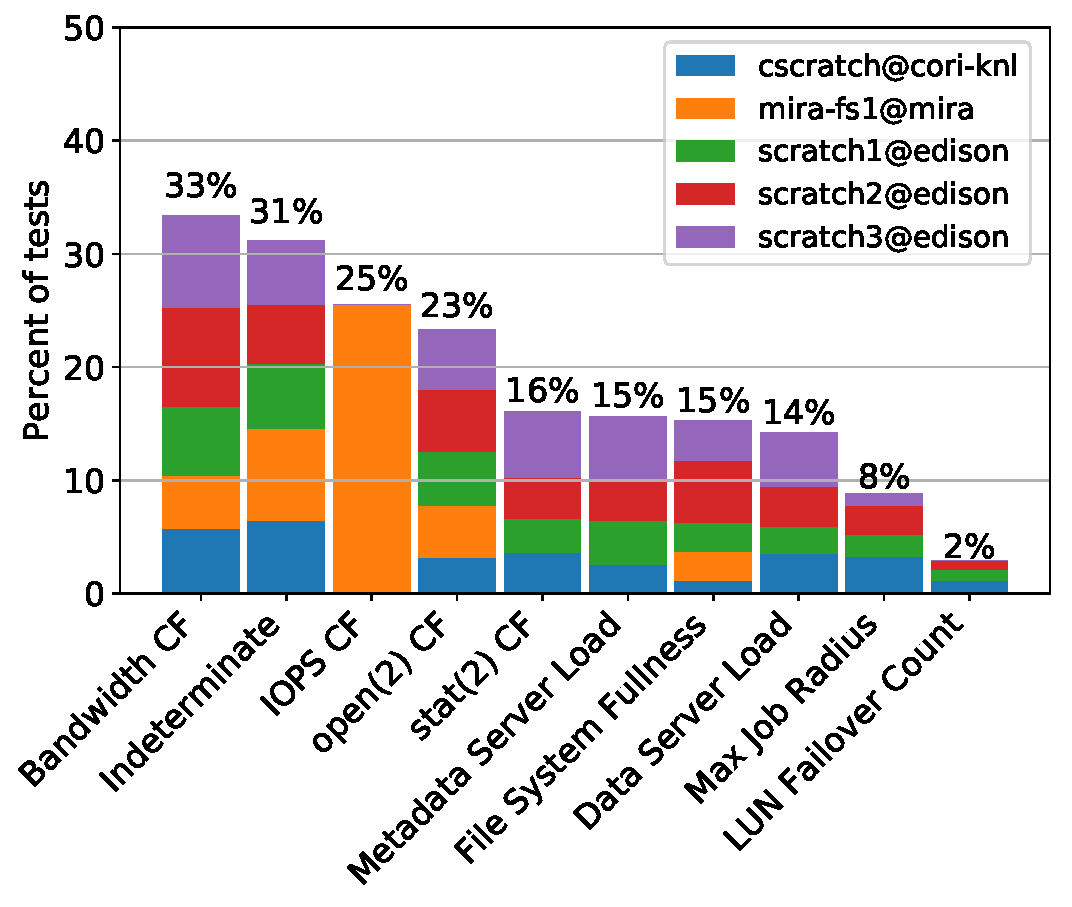
\includegraphics[width=1.0\columnwidth]{contributors-bad-by-system}
    \vspace{-.35in}
    \caption{Metrics that correlated with poor I/O performance across all file systems and benchmarks tested normalized to the number of probes during which each metric was measured.
    "CF" refers to coverage factor as defined earlier;
    "Indeterminate" are those jobs where no metrics could be classified as contributors.
    }
    \label{fig:contributors-bad-by-system}
    % source: sc18_umamify.ipynb
\end{figure}

As evidenced in Figures \ref{fig:summary-heatmap} and \ref{fig:regions-heatmap}, application performance is sometimes severely degraded for one and only one day in an otherwise unremarkable divergence region.
Furthermore, this performance loss may only be observed in one of the I/O motifs tested on that day, suggesting a very short-lived issue that disappeared over the course of one or two of the eight daily test jobs.
The lack of a gradual transition of performance around these transients results in a low-diversity set of observations that limits the confidence of correlation-based classification and places these events beyond the capabilities of the aforementioned correlative approach.

To classify these short-term cases, we apply a formalization of the UMAMI approach presented in earlier work~\cite{Lockwood2017}.
This method contextualizes the performance of a job of interest with respect to other jobs that (1) ran in the same period of time and (2) exhibited the same I/O motif to determine if its performance was truly abnormal given its divergence region.
Following this, other telemetric data (as described in Section \ref{sec:methods/tokio}) collected during each of the jobs sharing the same divergence region are also compared to determine the limits of normalcy for each metric.
By identifying all of the metrics which were statistically abnormal at the same time job performance was abnormal, we can establish a list of metrics that \emph{may have} contributed to that job's abnormal performance.

For this work, we partitioned each set of observations $J_{app, rw, sys}$ using $\textup{SMA}_{28}$ and $\textup{SMA}_{7}$ to establish divergence regions sufficiently small to capture individual performance transients.
Within each divergence region, the slowest performing day is then identified as a probe of interest, and each metric collected during that job's runtime is compared to the values measured during every other job in the same divergence region.
If the worst value of any given metric was observed at the same time the performance transient was observed, we flag that metric as being a possible contributor to the transient.
The result of this analysis is zero or more metrics being flagged as potential contributors to poor performance within each divergence region for each application, file system, and read/write mode.

Aggregating all of the divergence regions' contributors yields a broad overview of the metrics that most commonly coincide with poor performance across all of the test systems.
This distribution, shown in Figure \ref{fig:contributors-bad-by-system}, reveals that abnormally high bandwidth contention was found to coincide with abnormally poor performance most frequently.
IOPS contention, which was only measured on Mira, and the incidence of metadata 

\TODO{Define the metrics in Fig \ref{fig:contributors-bad-by-system}}